\begin{problem}%
{Ночь в музее}%
{\textsl{стандартный ввод}}%
{\textsl{стандартный вывод}}%
{1 секунда}%
{256 мегабайт}%
{}

Гриша, подобно персонажу известной кинокомедии, нашел себе ночную работу в музее естественной истории. В первую же смену ему выдали его главное орудие труда — \textit{эмбоссер} — и приказали провести инвентаризацию всей экспозиции.\\

\textit{Эмбоссер} представляет собой устройство для «печати» текста на пластиковой ленте. Текст набирается последовательно, буква за буквой. В устройство входят колесо с нанесёнными по кругу строчными буквами английского алфавита, неподвижная засечка, которая указывает на текущую букву, и кнопка, печатающая выбранную букву. За одно действие можно повернуть колесо с алфавитом на одну букву влево либо вправо по циклу. Изначально засечка эмбоссера указывает на букву a. Остальные буквы расположены так, как показано на рисунке.\\

\begin{center}
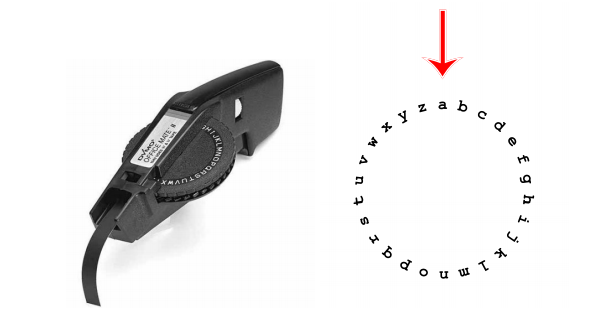
\includegraphics{images/2962.png}
\end{center}

После внесения предмета в базу Гриша должен с помощью эмбоссера выдавить на пластиковой ленте название и прикрепить его к экспонату. Возвращать колесо обратно в позицию, соответствующую букве a, не требуется.\\

Наш герой боится, что некоторые особо устрашающие экспонаты могут ожить и начать за ним свою охоту, поэтому он хочет как можно быстрее напечатать все названия. Помогите ему: для данного названия экспоната определите минимальное количество поворотов колеса, необходимое для его печати.

\InputFile

Единственная строка входных данных содержит название экспоната — строку, состоящую из не менее, чем одного, и не более, чем ста символов. Гарантируется, что строка состоит из строчных букв английского алфавита.

\OutputFile

Выведите единственное целое число — минимальное количество поворотов колеса, за которое Гриша сможет напечатать название экспоната.

\Examples

\begin{example}
\exmp{
zeus
}{%
18
}%
\exmp{
map
}{%
35
}%
\exmp{
ares
}{%
34
}%
\end{example}

\Explanation

\begin{center}
\begin{adjustbox}{max size={\textwidth}{\textheight}}
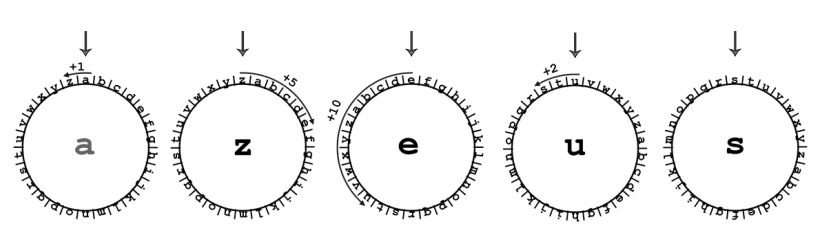
\includegraphics{images/2963.png}
\end{adjustbox}
\end{center}

Для набора слова из первого примера необходимо сделать следующую последовательность поворотов:

\begin{enumerate}
    \item от a до z ($1$ поворот против часовой стрелки),
    \item от z до e ($5$ поворотов по часовой стрелке),
    \item от e до u ($10$ поворотов против часовой стрелки),
    \item от u до s ($2$ поворотa против часовой стрелки).
\end{enumerate}

Итого потребуется $1$ + $5$ + $10$ + $2$ = $18$ поворотов.

\end{problem}
